\section{Värmeutveckling}
\index{värmeutveckling}
\index{heat dissipation}

\subsection{Värmeledning}
\textbf{
HAREC a.\ref{HAREC.a.2.7.1}\label{myHAREC.a.2.7.1}
}
\index{värmeledning}
\index{heat transfer}
\index{termisk resistans}
\index{symbol!\(R_\Theta\) termisk resistans}
\index{ambient temperature}
\index{symbol!\(T_A\) ambient temperature}
\index{elsäkerhet}
\index{kalllödning}

Vi har tidigare betraktat Joules lag för effektutveckling i motstånd.
Det är dags att börja utveckla en lite mer komplett syn på värme-utveckling.
Ett motstånd som utvecklar 1 Watt kommer stiga i temperatur tills dess att
värmeledningen förmår att avleda värmen.

För värmeavledning så är det temperatur-skillnaden som motsvarar spänning och
avledd effekt Watt (eller Joules per sekund) motsvarar störm. Den termiska
värmeledningsförmånga avgör helt enkelt hur hög temperatur-skillnad som behövs
för att avleda värmen. Ju högre effekt som skall avledas, ju högre temperatur-
skillnad krävs för uppnådd avkylning.

\emph{Termisk resistans} (eng. \emph{thermal resistance}) är ett mått på
motståndet att leda värme och har symbolen \(R_\Theta\), och är antalet grader
Kelvin per Watt. Temperaturen \(T_k\) för en kompontent bero på medel-effekten
\(P\) den producerar i värme, det termiska motståndet samt
\emph{omgivande temperatur} (eng. \emph{ambient temperature}) \(T_A\) enligt:

\(T_k = T_A + R_\Theta P\)

Det termiska motståndet kan summeras precis som vanligt motstånd, vilket kan
förstås med att det är samma effekt \(P\) som behöver kylas och temperatur-
skillnaden för varje steg kommer att addera sig.

\subsection{Konvektion}
\textbf{
HAREC a.\ref{HAREC.a.2.7.2}\label{myHAREC.a.2.7.2}
}
\index{konvektion}
\index{kylfläns}
\index{heatpipe}

\emph{Konvektion} (eng. \emph{convection}) är när värme skapar ett flöde i
gas eller vätska, oftast luft. När luft värms upp så vill den expandera, varvid
den tar större plats. Det är t.ex. den grundläggande lyft-principen hos en
varmlufts-ballong. Vid all värmealstring i elektronik uppstår konvektion, vilket
gör att varm luft flyttar sig uppåt varvid kallare luft kan komma till och
därmed kyla värmekällan. Ju större temperatur-skillnad, ju större lyft-kraft
hos en uppvärmda luften och därmed bättre kylning.

För t.ex. transistorer kan värmealstringen ske på en sådan koncentrerad yta att
konvektion inte räcker för att kyla den producerade värmen, och därför monterar
man dem på så kallade \emph{kylflänsar} (eng. \emph{heat sinks}) som leder ut
värmen till en större yta så att konvektionen får en chans att kyla.
En effektivare metod att transportera värme är så kallad \emph{heatpipe} (eng.
\emph{heat pipe}) där vätska i ett rör som effektivt flyttar överskottsvärme
från ett ställe till ett annat och därmed kyler. Det används numer ofta i
datorer.

Om värme produceras på för tät yta kan man behöva hjälpa konvektionen, vilket
ibland kallas för \emph{forcerad konvektion} (eng. \emph{forced convection}),
dvs. med hjälp av fläkt trycka luft mot kylflänsen och ibland även dra bort
den varma luften. Eftersom fläktar skapar oljud brukar man försöka begränsa
varvtalet beroende på temperaturen, men även variationen av varvtal kan
uppfattas som störande. Andra åtgärder för att minska störningarna är att
skapa släta vägar för luften så det inte blidas virvelvindar, och ibland att
styra luften med bafflar in och ut.

Ett problem som kan uppstå är att utrustning som är gjord för självkonvektion
kan bli ställd eller monterad så att luft inte kan flöda fritt för att kyla
den, det kan leda till överhettning. På motsvarande sätt kan en trasig fläkt
skapa överhättning. Dålig kontakt mellan transistor och kylfläns är ett annat
exempel på hur dålig värmeledning skapar överhettning.

\subsection{Värmealstring}
\textbf{
HAREC a.\ref{HAREC.a.2.7.4}\label{myHAREC.a.2.7.4}
}
\index{värmealstring}

\emph{Värmealstring} kan ske på fler ställen än motstånd. Vi har redan berört
ledare. Lite förenklat kan man säga att alla komponenter har mer eller mindre
förluster, som producerar värme. Genom komponentval kan vi undvika att
producera onödig värme, dels genom att ha lägre förluster, men även genom att
inte skapa onödigt stora strömmar. Lägre förluster skapar man genom att helt
enkelt ha bättre ledningsförmåga, lägre resistans. Det är dock för många
delar av designen högst försumbara förluster som inte kräver någon större
hänsyn för att få det överleva. Kraftaggregat och effekt-steg är dock sådana
ställen där det går större strömmar och ofrånkomligen där man också alstrar
värme.

Även halvledare skapar värme, och även här gäller Joules lag med spänning
gånger ström. I ett effektsteg t.ex. så kommer transistorn ``bränna'' av
effekten för spänningen över transistorn gånger strömmen genom transistorn.
Onödigt hög spänning ger därför onödigt hög förlust. På motsvarande sätt ger
onödigt hög ström onödigt hög förlust, vilket är en anledning till att man
gärna undviker Klass A steg till fördel för klass AB, B eller C.

Bristande värmeavledning leder ofta till katastrofalt fel, som t.ex.
sönderbrända motstånd och transistorer, men även ledare kan brinna av när man
har för smal ledare, och därmed för hög resistans, för den ström som skall gå
genom den och med tanke på dess förmåga att kyla av sig. Av det skälet finns
t.ex. krav på minsta arean (``kvadrat'') av koppar i ledare i
elsäkerhetsföreskrifter, helt enkelt för att de inte skall skapa brand.

En annan effekt av värmeledning är att det kan ibland vara svårt att löda på
kretskort, framförallt ledare som går mot stora kopparplan som ju har relativt
god värmeledningsförmåga. Ibland designar man små mönster ``thermals'' runt
sådana lödpunker för att minska värmeavledningen. Ett effektivt sätt att
kunna löda och framförallt löda av från sådana kort är att man förvärmer kortet
rejält runt om, för då kommer temperatur-skillnaden mellan lödpennans spets
och omgivningen att minska och därmed värmeledningen bort från lödpunkten och
då krävs det inte lika stor effekt att få upp lödpunkten i rätt temperatur för
att kunna smälta tennet och få det att stelna långsamt för en god lödning, dvs.
undvika ``kall-lödning''.

\subsection{Värme i transistor}
\textbf{
HAREC a.\ref{HAREC.a.2.7.3}\label{myHAREC.a.2.7.3}
}

För att förstå värmealstring i en transistor så börjar vi med att tänka oss
att vi har en transistor som matas med 12 V matspänning. Vi genererar då en
10 Vpp (topp-topp-spänning) sinus in i en last med 50 Ohm. Vad är effekt-
förlusten i transistorn?

\begin{figure}[h]
\begin{center}
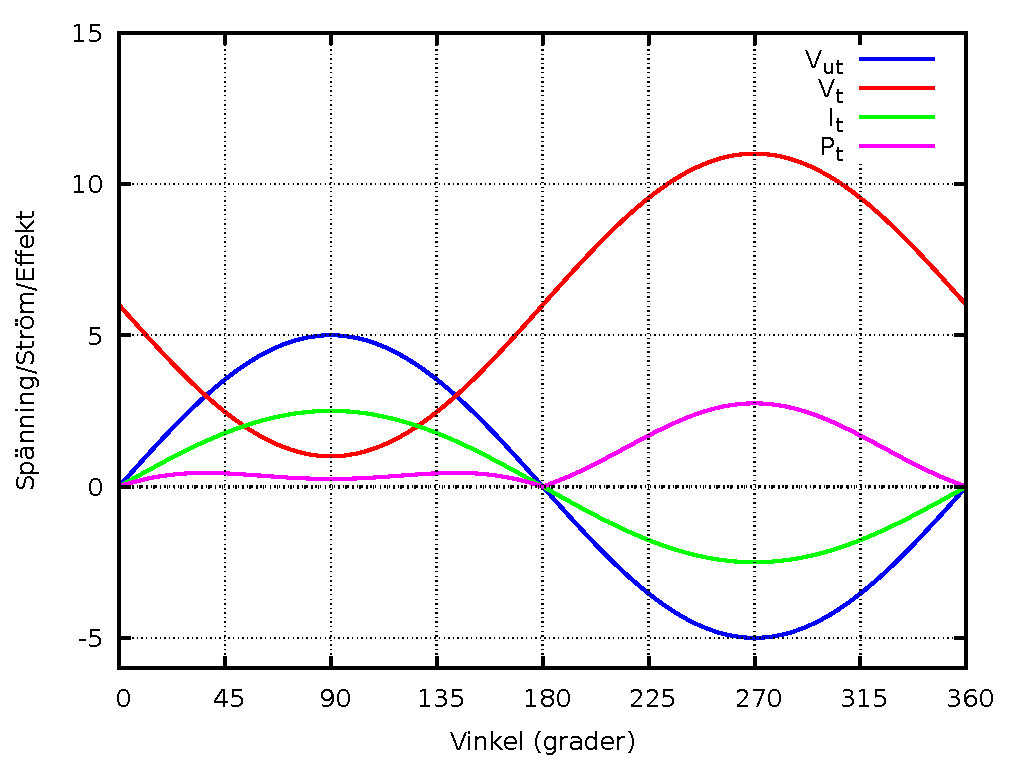
\includegraphics[width=7cm]{images/power1}
\caption{Utspänning $V_{ut}$, Transistor-spänning $V_t$, Transistor-ström $I_t$ och transistor-effekt $P_t$ varierar med vinkel sinus-signalen för resitiv last.}
\label{fig:power1}
\end{center}
\end{figure}

I bild \ref{fig:power1} ser vi utsignalen \(V_ut\) som en sinus med amplituden
\(5\ V\), dvs \(10\ V_{pp}\). Eftersom transistor har en vilo-spänning på 6 V
för att få marginal mot \(0\ V\) och \(+12\ V\), så kommer spänningen variera
mellan \(1\ V\) och \(11\ V\) och det ser man i \(V_t\) kurvan. Utgångslastens
resistor lastar med en ström \(I_t\) som är proportionelig mot spänningen
\(V_{ut}\) på utgången. Effekten för transistorn \(P_t\) är sedan absolut-
funktionen för strömmen gånger spänningen, dvs. Joules lag. Den observante ser
att effekten är signifikant högre för andra halvan av kurvan, då man har både
hög spänning och hög ström.
